\chapter{Results}
\label{chap:results}

This chapter starts with a qualitative reader map, then reports quantitative
results by city and profile before returning to the final aggregate averages.
The frozen prior results are reported on their own first: the channel
attenuation prior, the delay spread prior, and the angular spread prior. The
final \textsc{HARP-Net CKM} residual model is then compared with those frozen
priors on the unseen test cities. The standalone path loss prior audit uses the
city holdout validation+test pool: 5340 samples from 29 unseen cities. The
selected final model is evaluated on the final 2590-sample, 14-city test split.
Two path loss prior numbers therefore appear in this chapter:
\SI{1.9246}{dB} is the standalone calibrated hybrid prior on the held out
validation+test pool, whereas \SI{1.9383}{dB} is the frozen path loss prior
baseline used by \textsc{HARP-Net CKM} on the final 14-city test split. All
final model versus prior comparisons use the latter.

The evaluation mask, pixel weighted RMSE rule and map correlation definition
are given in Section~\ref{sec:evaluation_metrics}. All final numbers in this
chapter use that same valid receiver protocol.

The prior is one of the central results of the thesis: a strong baseline
calibrated only on training cities that absorbs the stable part of the map
before the residual model is asked to solve the harder local errors. This
chapter focuses on the frozen priors and final test evaluation.

\section{Qualitative Reader Map}
\label{sec:qualitative_reader_map}

Figure~\ref{fig:try80_panel_results} is placed before the tables because it is
the best compact explanation of the final method. The panel shows, for one
held out Vancouver sample, the same sequence used throughout the thesis: the
ray traced target, the frozen prior, the residual correction, the final
prediction and the remaining error. Reading the figure before the quantitative
sections makes the later tables less abstract: the reported RMSE gains are the
pixel aggregate version of the local corrections visible in the lower rows.

\begin{figure}[!htbp]
\centering
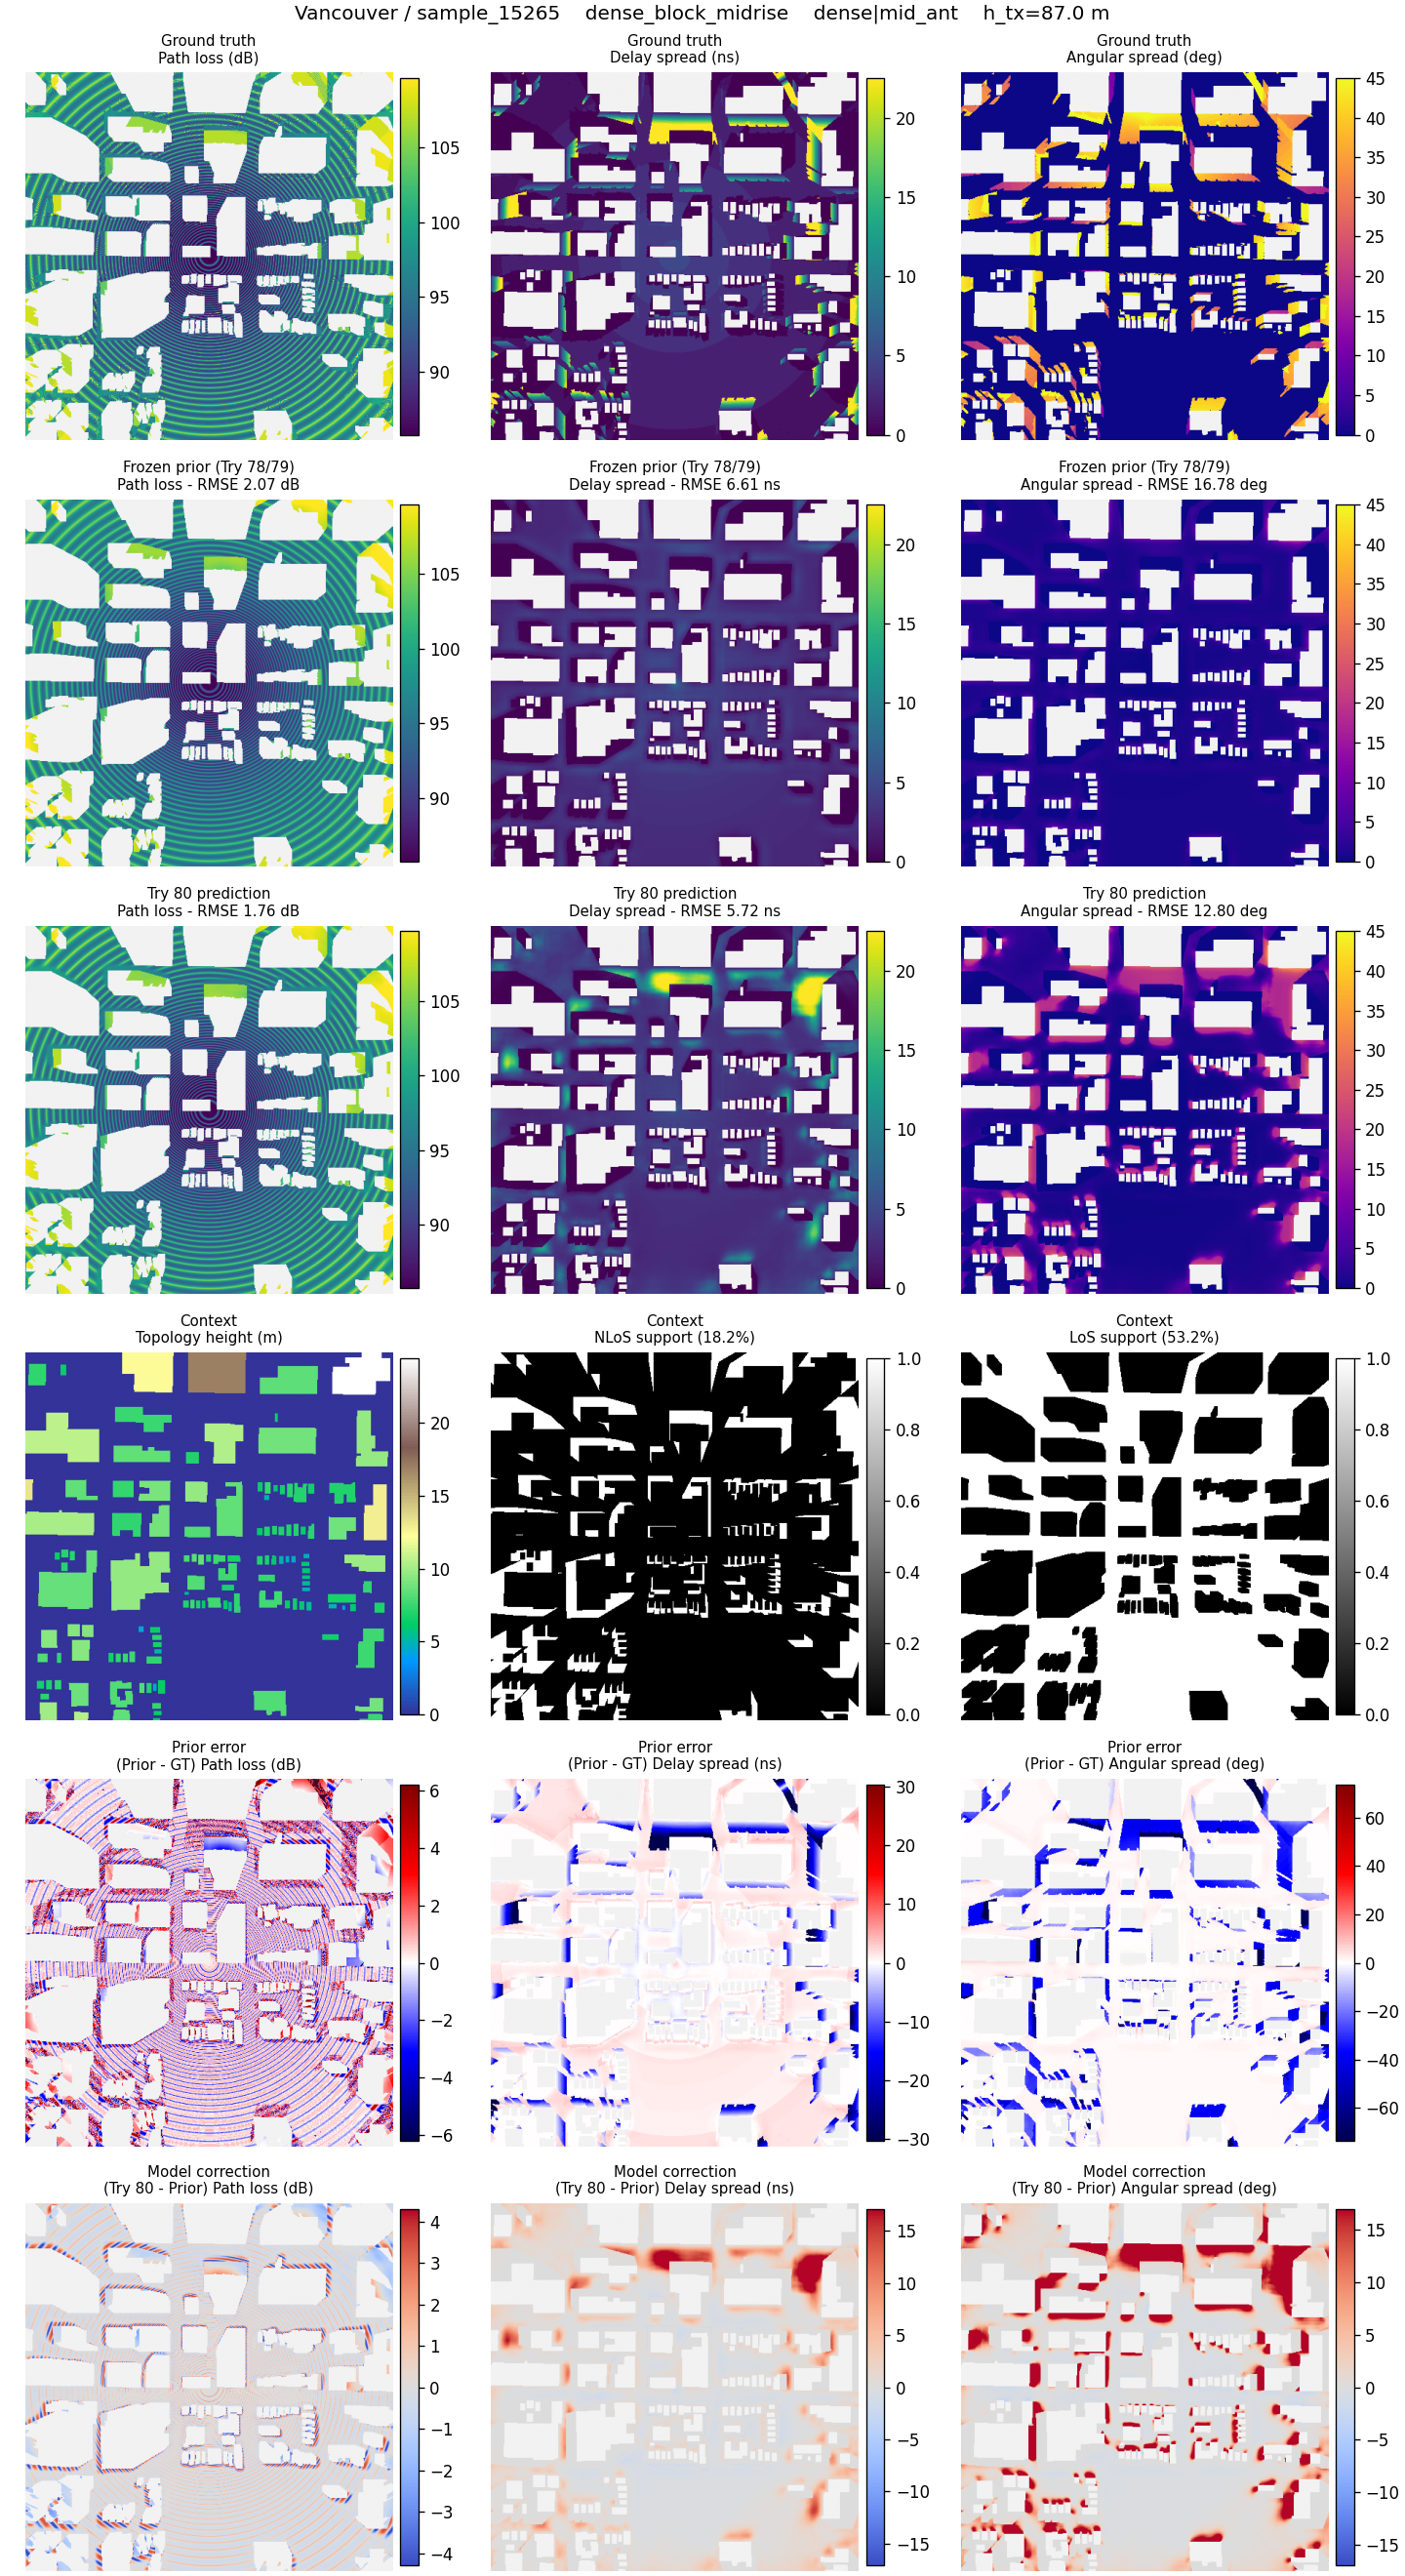
\includegraphics[width=\textwidth,height=0.78\textheight,keepaspectratio]{img/thesis_figures/try80_appendix_panels/try80_panel_dense_mid_ant_Vancouver_sample_15265_6x3.png}
\caption[Representative final model inspection panel.]%
{Representative final model inspection panel for a dense, mid altitude, held
out test sample in Vancouver. The panel shows the final prior, neural residual
correction and prediction side by side, making visible how
\textsc{HARP-Net CKM} improves a strong prior instead of replacing it.}
\label{fig:try80_panel_results}
\end{figure}

The important qualitative point is that the channel attenuation prior already
gets the large radial structure approximately right, especially in visible
regions. The neural model is therefore judged by whether it improves local
structure around building borders, blocked regions and spread tails. This is
why the following sections report not only one global average but also city,
topology, antenna height and visibility breakdowns.

\section{City and Profile Audit}
\label{sec:city_profile_audit}

The first quantitative view is deliberately by city rather than by global
average. The latest DirectML evaluation CSVs already store per city rows with
the final checkpoint and clipping rules, so no new evaluation is needed for this
audit. Training cities are intentionally not shown: they are useful for
debugging, but they are not a fair generalisation comparison because the priors
and residual model were fitted using those cities. Tables
\ref{tab:try80_val_city_audit} and \ref{tab:try80_test_city_audit} therefore
show validation and test cities only.

The last two columns give the percentage of samples in the three environment
groups and in the three antenna height groups. These proportions explain why
some cities are intrinsically harder than others before any global averaging is
done. The following sections then aggregate the same evaluation protocol by
frozen prior, topology, antenna height, LoS/NLoS state and final test average.

\begin{table}[!htbp]
\centering
\caption[\textsc{HARP-Net CKM} validation RMSE by city.]%
{\textsc{HARP-Net CKM} validation RMSE by city. Attenuation is in dB, delay
spread in ns and angular spread in degrees. The topology mix column is
open/mixed/dense; the height mix column is low/mid/high antenna percentage.}
\label{tab:try80_val_city_audit}
\scriptsize
\begin{tabularx}{\textwidth}{>{\raggedright\arraybackslash}Xrrrrcc}
\toprule
City & Samples & Att. & Delay & Angular & Topology mix & Height mix \\
\midrule
Bilbao & 50 & 2.02 & 41.7 & 13.0 & 10/60/30 & 26/38/36 \\
Chiang Mai & 95 & 2.06 & 38.9 & 13.7 & 5/74/21 & 38/31/32 \\
Cleveland & 150 & 1.61 & 19.7 & 12.1 & 30/67/3 & 37/27/35 \\
Dhaka & 225 & 1.79 & 36.2 & 12.1 & 22/36/42 & 26/36/38 \\
Dubrovnik & 90 & 1.24 & 23.5 & 10.2 & 72/28/0 & 40/32/28 \\
Fortaleza & 345 & 1.47 & 11.7 & 11.0 & 14/23/62 & 32/30/38 \\
Marrakesh & 75 & 1.26 & 17.0 & 8.7 & 53/47/0 & 33/25/41 \\
Mexico City & 650 & 1.91 & 21.9 & 11.9 & 7/26/67 & 32/36/32 \\
Munich & 140 & 1.80 & 28.2 & 12.4 & 11/64/25 & 26/39/35 \\
Nazareth & 105 & 1.51 & 26.4 & 12.0 & 52/43/5 & 37/30/32 \\
Nice & 35 & 1.65 & 20.3 & 11.2 & 14/43/43 & 14/46/40 \\
Salvador & 105 & 1.90 & 22.4 & 12.5 & 14/29/57 & 36/30/34 \\
Segovia & 30 & 1.12 & 14.2 & 7.2 & 67/17/17 & 30/30/40 \\
Tunis & 400 & 1.32 & 10.7 & 10.5 & 18/38/45 & 37/29/34 \\
Victoria & 255 & 1.54 & 13.1 & 10.6 & 35/65/0 & 30/35/35 \\
\bottomrule
\end{tabularx}
\end{table}

\begin{table}[!htbp]
\centering
\caption[\textsc{HARP-Net CKM} test RMSE by city.]%
{\textsc{HARP-Net CKM} test RMSE by city. Attenuation is in dB, delay spread
in ns and angular spread in degrees. The topology mix column is
open/mixed/dense; the height mix column is low/mid/high antenna percentage.}
\label{tab:try80_test_city_audit}
\scriptsize
\begin{tabularx}{\textwidth}{>{\raggedright\arraybackslash}Xrrrrcc}
\toprule
City & Samples & Att. & Delay & Angular & Topology mix & Height mix \\
\midrule
Barcelona & 50 & 1.74 & 33.0 & 11.0 & 30/30/40 & 40/32/28 \\
Beijing & 200 & 1.57 & 23.3 & 10.5 & 28/65/8 & 30/41/30 \\
Carcassonne & 110 & 1.43 & 8.0 & 9.6 & 41/50/9 & 30/29/41 \\
Copenhagen & 220 & 1.83 & 27.3 & 11.9 & 14/68/18 & 37/27/36 \\
Halifax & 250 & 1.43 & 19.9 & 9.6 & 78/22/0 & 36/33/31 \\
Jaipur & 120 & 2.05 & 21.6 & 11.9 & 12/25/62 & 37/34/29 \\
Johannesburg & 245 & 1.76 & 21.0 & 12.1 & 10/55/35 & 34/34/32 \\
Key West & 105 & 1.39 & 20.0 & 10.4 & 52/43/5 & 33/30/37 \\
Kuala Lumpur & 360 & 2.05 & 44.2 & 13.3 & 18/44/38 & 29/38/34 \\
Osaka & 50 & 2.43 & 37.3 & 14.5 & 0/60/40 & 28/44/28 \\
Phuket & 50 & 1.82 & 37.2 & 13.7 & 20/50/30 & 28/36/36 \\
Pune & 135 & 1.95 & 33.3 & 13.1 & 15/67/19 & 32/27/41 \\
Surat & 190 & 1.63 & 23.5 & 10.2 & 34/16/50 & 36/32/32 \\
Vancouver & 505 & 1.53 & 17.7 & 10.7 & 29/67/4 & 31/35/34 \\
\bottomrule
\end{tabularx}
\end{table}

The per city rows show why a single average is not enough. Osaka, Kuala Lumpur
and Phuket are visibly harder than Halifax or Carcassonne, especially for delay
spread, and this is consistent with their city mix and height composition. The
aggregate tables later in the chapter should therefore be read as summaries of
this city distribution, not as a replacement for it.

\section{Standalone Frozen Prior Results}

\subsection{Prior audit protocol and headline results}

The final path loss prior is the clearest evidence that the prior is a strong
path loss baseline in its own right. Its LoS branch reaches
\SI{1.7516}{dB} RMSE, and the final hybrid prior reaches
\SI{1.9246}{dB} overall under the pixel weighted metric on the held out
validation+test pool.

The spread priors are evaluated on the final city holdout test split because
they are the baselines used by the final residual model. Delay spread reaches
\SI{28.10}{ns} RMSE, and angular spread reaches \(13.74^\circ\) RMSE before
any neural correction. The detailed rows below use the same valid receiver
masking rule as Section~\ref{sec:evaluation_metrics}.

\subsection{Channel attenuation prior result}

The path loss prior is reported here in its final hybrid form. The relevant
result for this chapter is the frozen calibrated prior that is later used as
the anchor for \textsc{HARP-Net CKM}.

\paragraph{Split comparability note.}
The final priors and \textsc{HARP-Net CKM} use the same \texttt{city\_holdout}
split with \texttt{val\_ratio = 0.15}, \texttt{test\_ratio = 0.15}, and
\texttt{split\_seed = 42}. The standalone path loss prior audit uses the
training cities and the full validation+test held out pool, giving
\SI{1.9246}{dB} over 5340 held out samples. The final model comparison remains
test only, so the frozen path loss prior baseline in
Table~\ref{tab:try80_final_test_overall} is \SI{1.9383}{dB}.

The calibrated attenuation prior is the strongest non neural baseline in the
thesis. It is split into LoS and NLoS branches because those regimes have
different error mechanisms, but the construction details belong to
Chapter~\ref{chap:methodology}. In this chapter the prior is used as a frozen
baseline for the final test comparison.

The final reporting separates LoS and NLoS wherever the target definition
allows it. A single overall number can hide whether the model is improving
direct visibility pixels, blocked pixels, or only the easier majority regime.

\begin{table}[!htbp]
\centering
\caption{Final hybrid path loss prior, pixel weighted RMSE on the
held out validation+test split.}
\label{tab:pl_prior_results}
\begin{tabular}{lcc}
\toprule
Region & RMSE & Unit \\
\midrule
LoS & 1.7516 & dB \\
NLoS & 3.3967 & dB \\
Overall & 1.9246 & dB \\
\bottomrule
\end{tabular}
\end{table}

\subsection{Angular spread prior result}

The same calibrated spread prior module is used for angular spread and delay
spread, so Table~\ref{tab:spread_prior_results} reports both targets together
before the next two subsections interpret them separately. A large part of the
spread targets can already be explained by geometry, building layout, and
calibration without a neural network. The fitted calibration dictionary contains
\(114\) case keys, but this number is not one simple Cartesian product. For each
spread metric, the exact grid has
\(6\) topology classes \(\times\) \(2\) LoS/NLoS states \(\times\) \(3\)
antenna height bins, or \(36\) exact keys. The implementation then adds
fallback calibrations for sparse cases: \(12\) antenna collapsed topology
and LoS/NLoS keys, \(6\) topology wide keys, \(2\) global LoS/NLoS keys, and
\(1\) fully global key. This gives \(57\) keys per spread metric and
\(114\) keys across delay spread and angular spread. Equivalently, the
dictionary contains \(72\) exact DS/AS cases plus \(42\) fallback cases.
The point of this dictionary is not novelty by formula alone, but coverage: the
baseline is strong because it stores many small regime specific decisions about
density, building height, visibility, and antenna height instead of forcing one
global estimator to explain all pixels.
The calibrated spread prior module applies this idea separately to delay spread and angular spread. The
raw spread estimate is only the first feature; the calibrated model then uses a
23-term vector with raw prior curvature, range, elevation angle, transmitter height,
local building density at two scales, local height at two scales, LoS/NLoS
support at two scales, blocker depth, transmitter clearance, taller building
fraction, and interaction terms. Both spread targets are fitted in
\(\log(1+y)\) space, so the model can handle the LoS spike near zero and the
long NLoS tail with one calibrated framework while still reporting metrics in
native ns and degrees.

\begin{table}[!htbp]
\centering
\caption{Calibrated spread prior test results, pixel weighted RMSE.}
\label{tab:spread_prior_results}
\begin{tabular}{lccc}
\toprule
Metric & Overall & LoS & NLoS \\
\midrule
Delay spread (ns) & 28.10 & 27.49 & 29.62 \\
Angular spread ($^\circ$) & 13.74 & 15.28 & 8.66 \\
\bottomrule
\end{tabular}
\end{table}

For angular spread, the calibrated prior already reaches \(13.74^\circ\)
overall RMSE on the unseen test split, below the original \(20^\circ\) project
target. The LoS row is harder than the NLoS row (\(15.28^\circ\) versus
\(8.66^\circ\)), which indicates that the challenge is not only blockage: local
angular variation in visible streets also remains important.

\subsection{Delay spread prior result}

For delay spread, the calibrated prior reaches \SI{28.10}{ns} overall RMSE,
also below the original \SI{50}{ns} project target. Its LoS and NLoS rows are
closer than in angular spread (\SI{27.49}{ns} and \SI{29.62}{ns}), but the
largest residual errors still come from rare high delay regions. This is why the
final residual model is evaluated not only by RMSE but also by MapCorr.

\subsection{Prior height and topology checks}

The CKM dataset covers stored transmitter heights from about \SI{12}{m} to almost
\SI{478}{m}, while the generator distribution has support up to
\SI{500}{m}. The absence of samples above \SI{478}{m} is statistically normal
for this finite draw, because the expected count above that height is only
0.52. Therefore the conditional error at a single aggregate RMSE can hide
strong altitude-dependent structure. Tables~\ref{tab:pl_prior_by_height} and
\ref{tab:spread_prior_by_height} therefore break the path loss prior and the
delay spread and angular spread priors into four transmitter height bins, using the
same pixel weighted aggregation as the headline tables.

\begin{table}[!htbp]
\centering
\caption{Path loss prior pixel weighted RMSE by transmitter height, on
the held out validation+test split.}
\label{tab:pl_prior_by_height}
\small
\begin{tabularx}{\textwidth}{>{\raggedright\arraybackslash}Xrrrr}
\toprule
Transmitter height bin & Overall & LoS & NLoS & Samples \\
\midrule
12 to 50   & 2.180 & 1.797 & 3.756 & 1211 \\
50 to 150  & 1.936 & 1.785 & 3.228 & 2634 \\
150 to 300 & 1.680 & 1.666 & 2.259 &  786 \\
300 to 500 & 1.627 & 1.619 & 2.255 &  362 \\
\bottomrule
\end{tabularx}
\end{table}

\begin{table}[!htbp]
\centering
\caption{Delay spread and angular spread calibrated pixel weighted RMSE
by transmitter height, on the city holdout test split.}
\label{tab:spread_prior_by_height}
\small
\begin{tabularx}{\textwidth}{>{\raggedright\arraybackslash}Xlrrr}
\toprule
Transmitter height bin & Metric & Overall & LoS & NLoS \\
\midrule
12 to 50   & Delay spread (ns)       & 39.90 & 43.04 & 35.13 \\
50 to 150  & Delay spread (ns)       & 27.17 & 26.72 & 28.29 \\
150 to 300 & Delay spread (ns)       &  8.70 &  8.79 &  8.13 \\
300 to 500 & Delay spread (ns)       &  3.70 &  3.80 &  2.76 \\
\midrule
12 to 50   & Angular spread ($^\circ$) & 15.69 & 18.81 &  9.93 \\
50 to 150  & Angular spread ($^\circ$) & 14.19 & 15.89 &  8.41 \\
150 to 300 & Angular spread ($^\circ$) & 10.39 & 11.07 &  4.49 \\
300 to 500 & Angular spread ($^\circ$) &  8.85 &  9.34 &  2.85 \\
\bottomrule
\end{tabularx}
\end{table}

The altitude dependence is monotonic and physically intuitive. Higher UAV
transmitters see more of the ground as unobstructed LoS and encounter fewer
deep shadow pockets, so both the NLoS pixel fraction and the worst-case tails
shrink. Path loss NLoS RMSE drops from \SI{3.76}{dB} at low altitudes to
\SI{2.26}{dB} above \SI{300}{m}, and delay spread NLoS RMSE collapses from
\SI{35.13}{ns} to \SI{2.76}{ns} in the same comparison. The opposite is true
for the absolute number of samples: the dataset is dominated by the
\SI{50}{\mathrm{-}}\SI{150}{m} band, so the global aggregate RMSE reflects that
regime more than the higher-altitude extremes. Together with the empirical HDF5
histogram of \eqref{eq:height_empirical_histogram} and the counts reported in
Chapter~\ref{chap:methodology}, this means the high altitude rows are better
despite having much less training support, not because they are
over represented in the dataset. A practical consequence for
the final residual model is that the neural residual head has less to correct at high altitudes,
where the path loss prior is already close to the quantisation floor. The
remaining headroom lives in the low altitude, NLoS heavy bin, which is exactly
where a distribution aware residual can matter.

\subsubsection{Path loss prior by topology class}

The headline path loss prior number (\SI{1.92}{dB} overall RMSE on the
held out validation+test split, see Table~\ref{tab:pl_prior_results}) hides the
same building layout structure captured by the topology aware breakdown. The per sample evaluation
records were aggregated again by classifying each evaluated sample into the six
topology classes with the same final routing rule. The pixel weighted RMSE per topology class is
reported in Table~\ref{tab:pl_prior_by_topology}.

\begin{table}[!htbp]
\centering
\caption[Hybrid path loss prior RMSE by topology class.]%
{Hybrid path loss prior, pixel weighted RMSE on the
held out validation+test split, broken down by topology class. The
overall row reproduces the RMSE values in Table~\ref{tab:pl_prior_results}; the
sample count is the sum of samples assigned to the six topology classes. The
aggregate prior evaluator contains 4994 topology assigned samples.}
\label{tab:pl_prior_by_topology}
\footnotesize
\begin{tabularx}{\textwidth}{>{\raggedright\arraybackslash}Xrrrr}
\toprule
Topology class & LoS & NLoS & Overall & Samples \\
\midrule
open sparse lowrise   & 1.39 & 2.92 & 1.43 &  895 \\
open sparse vertical  & 1.43 & 3.91 & 1.55 &  370 \\
mixed compact lowrise & 1.81 & 2.91 & 1.90 & 1240 \\
mixed compact midrise & 1.91 & 3.84 & 2.21 & 1060 \\
dense block midrise   & 2.19 & 3.20 & 2.40 & 1325 \\
dense block highrise  & 2.44 & 4.09 & 2.97 &  104 \\
\midrule
\textbf{Overall}        & \textbf{1.75} & \textbf{3.40} & \textbf{1.92} & \textbf{4994} \\
\bottomrule
\end{tabularx}
\end{table}

The LoS dependency on building layout is monotonic. The two-ray prior fits its
own ground reflection ring against an LoS marginal whose width grows with city
density and building height, so the LoS RMSE of the analytic model rises from
\SI{1.39}{dB} in the open sparse lowrise class to
\SI{2.44}{dB} in the dense block highrise class. The NLoS branch is less
ordered by building layout: the best NLoS topology class is
\emph{mixed compact lowrise} at \SI{2.91}{dB}, while the worst is
\emph{dense block highrise} at \SI{4.09}{dB}. The dataset is also unbalanced in
this respect: dense block highrise contributes only 104 of
the 4994 topology assigned evaluation samples, so its high RMSE has a relatively small impact
on the overall pixel weighted aggregate but is the regime most likely
to limit deployment in dense urban environments.

This topology breakdown also makes the central methodological claim of the
thesis quantitative. The prior calibrated only on training cities is not only
strong on average, but also auditable by city type and LoS/NLoS case. The longer comparison with
the historical development models is kept in Appendix~\ref{app:detailed_attempt_log}.

\subsubsection{Spread priors by topology class}

The delay spread and angular spread priors are also topology dependent. These
tables use the same city holdout test split as Table~\ref{tab:spread_prior_results}
and keep the dense pixel weighted metric separated by visibility regime.

\begin{table}[!htbp]
\centering
\caption{Delay spread prior RMSE by topology class on the city holdout test split.}
\label{tab:ds_topo}
\small
\begin{tabularx}{\textwidth}{>{\raggedright\arraybackslash}Xrrr}
\toprule
Topology class & Overall & LoS & NLoS \\
\midrule
open sparse lowrise   & 16.88 & 17.01 & 15.43 \\
open sparse vertical  & 40.84 & 40.44 & 44.08 \\
mixed compact lowrise & 17.27 & 16.65 & 18.91 \\
mixed compact midrise & 37.88 & 38.26 & 37.25 \\
dense block midrise   & 26.90 & 29.00 & 25.02 \\
dense block highrise  & 43.52 & 40.16 & 45.08 \\
\midrule
\textbf{Overall}      & \textbf{28.10} & \textbf{27.49} & \textbf{29.62} \\
\bottomrule
\end{tabularx}
\end{table}

\begin{table}[!htbp]
\centering
\caption{Angular spread prior RMSE by topology class on the city holdout test split.}
\label{tab:as_topo}
\small
\begin{tabularx}{\textwidth}{>{\raggedright\arraybackslash}Xrrr}
\toprule
Topology class & Overall & LoS & NLoS \\
\midrule
open sparse lowrise   & 10.01 & 10.30 & 6.33 \\
open sparse vertical  & 12.70 & 12.98 & 9.97 \\
mixed compact lowrise & 14.37 & 15.99 & 8.17 \\
mixed compact midrise & 15.26 & 17.85 & 9.57 \\
dense block midrise   & 15.53 & 21.20 & 8.17 \\
dense block highrise  & 14.64 & 21.33 & 9.78 \\
\midrule
\textbf{Overall}      & \textbf{13.74} & \textbf{15.28} & \textbf{8.66} \\
\bottomrule
\end{tabularx}
\end{table}

The spread priors show a different topology pattern from channel attenuation.
Delay spread is hardest in open sparse vertical and dense block highrise
settings, while angular spread is dominated by the LoS rows of denser classes.
This supports the final design choice to keep separate residual outputs for the
three targets instead of treating all CKM maps as one generic image regression
problem.

\section{\textsc{HARP-Net CKM} Results Against Frozen Priors}

\subsection{Final test protocol and grouped profiles}

\textsc{HARP-Net CKM} freezes the attenuation and spread priors and learns a bounded residual correction
for the three radio maps. It is tested on the city holdout test split with
2590 samples from 14 cities that were not seen in training. The model should
be read as a two stage final
pipeline, not only as the last fine tuning loss:
the large capacity probabilistic residual stage keeps NLL, KL, moment matching and
outlier budget terms active, while the reported checkpoint is the state
selected on validation after the deterministic RMSE/MAE dominant
fine tuning stage. The exact weights of both stages are listed in
Table~\ref{tab:try80_loss_settings}. The final claim is therefore an RMSE
improvement over the frozen priors rather than a calibrated probabilistic
prediction claim. The pixel weighted RMSE rule in \eqref{eq:rmse} is used for
the model and for the frozen priors.
Therefore \texttt{model\_rmse} in the evaluation JSON is target specific: it is the RMSE
for channel attenuation, delay spread, or angular spread individually, not a sum of the
three RMSE values. The three targets are kept separate because their units are
incompatible. Delay spread and angular spread are evaluated exactly like channel
attenuation: for each valid ground receiver pixel, the predicted value is
compared with the ray-traced CKM ground truth value, and the RMSE is accumulated
over all valid ground receivers.

\begin{table}[!htbp]
\centering
\caption[\textsc{HARP-Net CKM} held out test RMSE by topology.]%
{\textsc{HARP-Net CKM} held out test RMSE by six class topology. Each
\(\Delta\) column is model minus frozen prior, so negative is better.}
\label{tab:try80_final_test_topology}
\scriptsize
\begin{tabularx}{\textwidth}{>{\raggedright\arraybackslash}Xrrrrrrr}
\toprule
Topology class & Samples & PL & \(\Delta\)PL & DS & \(\Delta\)DS & AS & \(\Delta\)AS \\
\midrule
\texttt{dense\_block\_highrise} & 55 & 2.8960 & -0.1790 & 42.03 & -1.48 & 12.43 & -2.21 \\
\texttt{dense\_block\_midrise} & 505 & 2.2449 & -0.2244 & 25.63 & -1.27 & 12.79 & -2.74 \\
\texttt{mixed\_compact\_lowrise} & 670 & 1.6974 & -0.2472 & 16.70 & -0.67 & 11.80 & -2.57 \\
\texttt{mixed\_compact\_midrise} & 620 & 2.0068 & -0.2556 & 35.75 & -2.13 & 12.79 & -2.47 \\
\texttt{open\_sparse\_lowrise} & 520 & 1.2156 & -0.2401 & 16.41 & -0.49 & 8.29 & -1.73 \\
\texttt{open\_sparse\_vertical} & 220 & 1.2518 & -0.3086 & 38.37 & -2.47 & 10.91 & -1.79 \\
\bottomrule
\end{tabularx}
\end{table}

\begin{table}[!htbp]
\centering
\caption[\textsc{HARP-Net CKM} held out test RMSE by antenna height bin.]%
{\textsc{HARP-Net CKM} held out test RMSE by antenna height bin. Each
\(\Delta\) column is model minus frozen prior, so negative is better.}
\label{tab:try80_final_test_antenna}
\scriptsize
\begin{tabular}{lrrrrrrr}
\toprule
Antenna bin & Samples & PL & \(\Delta\)PL & DS & \(\Delta\)DS & AS & \(\Delta\)AS \\
\midrule
\texttt{low\_ant} & 846 & 1.8755 & -0.2645 & 35.33 & -2.02 & 13.15 & -2.36 \\
\texttt{mid\_ant} & 878 & 1.7382 & -0.2527 & 27.70 & -1.40 & 11.92 & -2.54 \\
\texttt{high\_ant} & 866 & 1.4990 & -0.2165 & 11.78 & -0.46 & 8.81 & -2.08 \\
\bottomrule
\end{tabular}
\end{table}

Tables~\ref{tab:try80_final_test_topology} and
\ref{tab:try80_final_test_antenna} show that the residual correction is not an
artifact of the global average. All six topology classes improve in RMSE for
all three outputs, and all three antenna height bins improve in RMSE for all
three outputs. The hardest cases are also physically plausible: dense high rise
maps remain the hardest channel attenuation case, while delay spread is largest
in low altitude and sparse vertical or mixed mid rise regimes where long
multipath tails are more frequent. The same grouped CSV shows positive
MapCorr gains for every topology class and every antenna bin; the largest
structural gains are for the two spread targets rather than for channel
attenuation.

\begin{table}[!htbp]
\centering
\caption{\textsc{HARP-Net CKM} test RMSE separated by LoS and NLoS pixels. The test
cities are unseen during training.}
\label{tab:try80_final_test_los_nlos}
\scriptsize
\begin{tabular}{llrrr}
\toprule
Target & Scope & Model RMSE & Prior RMSE & \(\Delta\) RMSE \\
\midrule
Attenuation & LoS & 1.5175 & 1.7519 & -0.2344 \\
Attenuation & NLoS & 3.1596 & 3.5143 & -0.3547 \\
Delay spread & LoS & 25.6137 & 27.5119 & -1.8983 \\
Delay spread & NLoS & 29.2464 & 29.6157 & -0.3693 \\
Angular spread & LoS & 12.5270 & 15.3751 & -2.8481 \\
Angular spread & NLoS & 8.4550 & 8.6614 & -0.2064 \\
\bottomrule
\end{tabular}
\end{table}

\subsection{Final aggregate test result}

The grouped profile tables lead to the final aggregate metrics in
Table~\ref{tab:try80_final_test_overall}. The aggregate is reported last in
this block because it is a summary of the city, topology, antenna and visibility
profiles above, not a replacement for them.

\begin{table}[!htbp]
\centering
\caption[\textsc{HARP-Net CKM} test results on unseen cities.]
{\textsc{HARP-Net CKM} test results on unseen cities, compared with the frozen
priors. Negative \(\Delta\) RMSE means that the model improves the prior.}
\label{tab:try80_final_test_overall}
\scriptsize
\begin{tabular}{lrrrrl}
\toprule
Target & Model RMSE & Prior RMSE & \(\Delta\) RMSE & Model MAE & Unit \\
\midrule
Attenuation & 1.6947 & 1.9383 & -0.2436 & 0.9772 & dB \\
Delay spread & 26.6882 & 28.1211 & -1.4329 & 7.8160 & ns \\
Angular spread & 11.5253 & 13.8162 & -2.2909 & 4.8899 & \(^{\circ}\) \\
\bottomrule
\end{tabular}
\end{table}

\begin{table}[!htbp]
\centering
\caption[Engineering reading of the final Try 80 RMSE values.]%
{Engineering reading of the final Try 80 RMSE values. The broad targets are the
initial project acceptance thresholds; the final interpretation also considers
the frozen prior and the structural metrics in Table~\ref{tab:try80_final_test_mapcorr}.}
\label{tab:try80_final_engineering_judgement}
\scriptsize
\begin{tabularx}{\textwidth}{l>{\raggedright\arraybackslash}X>{\raggedright\arraybackslash}X>{\raggedright\arraybackslash}X}
\toprule
Output & Broad target & Current Try 80 test RMSE & Judgment \\
\midrule
Attenuation &
\(<\SI{5}{dB}\) &
\SI{1.6947}{dB} overall; \SI{3.1596}{dB} NLoS &
Excellent overall, and still good in the harder NLoS pixels. \\
Delay spread &
\(<\SI{50}{ns}\) &
\SI{26.6882}{ns} overall &
Good as scalar RMSE, with remaining spatial difficulty visible in MapCorr. \\
Angular spread &
\(<\SI{20}{\degree}\) &
\(11.5253^\circ\) overall; \(8.4550^\circ\) NLoS &
Good overall, especially in NLoS where angular dispersion matters most. \\
\bottomrule
\end{tabularx}
\end{table}

Under this evaluation protocol, the attenuation result is the clearest final
success. The original \SI{5}{dB} target remains defensible as a broad project
requirement, but it is no longer the most informative benchmark: Try 78 already
provided a frozen attenuation prior below \SI{2}{dB}. The relevant final
question is therefore whether the neural residual model improves that prior
without damaging the map structure. It does: RMSE falls from \SI{1.9383}{dB}
to \SI{1.6947}{dB}, and MapCorr rises from \(0.947710\) to \(0.961055\).
This is not directly comparable with easier radio map challenge scores that use
fixed transmitter heights, random splits, different clipping or different
building masks, but it is very strong for strict city holdout, continuous UAV
height conditioning and full \(513\times513\) CKM maps.

The spread numbers should be read differently. The reviewed literature rarely
reports dense per pixel delay spread or angular spread maps over unseen cities
with the same inputs. Their strongest interpretation is therefore internal to
this thesis and within the same protocol: both targets beat the project
thresholds and both improve over the frozen priors. The RMSE changes are
modest for delay spread and clearer for angular spread, while MapCorr improves
much more strongly for both. This means that Try 80 is not merely moving the
global mean of the spread maps; it is better locating the relative high and low
dispersion regions inside each city.

The physical meaning of the three RMSE values is also different. For channel
attenuation, an error of \(e\) dB corresponds to a multiplicative received
power uncertainty of
\begin{equation}
  G(e) = 10^{e/10}.
\end{equation}
Thus \SI{1.6947}{dB} corresponds to a factor of \(10^{1.6947/10}=1.48\),
whereas the original \SI{5}{dB} target corresponds to a factor of
\(10^{5/10}=3.16\). Near a coverage boundary, a \SI{5}{dB} error is therefore
not a small perturbation: it can change outage decisions, link margin, MCS
selection or handover regions. The final \SI{1.6947}{dB} value is much smaller,
corresponding to a factor of about \(1.48\times\), so the remaining global
attenuation uncertainty is close to the one dB quantization scale of the stored
maps. This is why the final attenuation result is the strongest claim in the
thesis: it is far below the original engineering target and improves a frozen
prior that was already below \SI{2}{dB}. For delay spread,
the same RMSE value can be translated into an equivalent excess propagation
length,
\begin{equation}
  \Delta d = c\,\Delta \tau,
\end{equation}
where \(c=0.299792458~\mathrm{m/ns}\). The final
\SI{26.6882}{ns} delay spread RMSE therefore corresponds to
\(0.299792458\times 26.6882=\SI{8.00}{m}\), while the original
\SI{50}{ns} target corresponds to \SI{14.99}{m}. This means that the typical
error in RMS temporal dispersion is on the scale of the delay produced by
about \SI{8}{m} of additional multipath path length. It does not mean that each
ray path is wrong by \SI{8}{m}; it gives the physical scale of the remaining
uncertainty in the temporal dispersion of the multipath channel. For angular
spread, the LoS and NLoS rows are more informative than the global average.
LoS angular spread can be dominated by the direct ray plus narrow reflected
components, so small angular spikes can be numerically visible without being
the most critical link level effect. NLoS angular spread is more communication
relevant because it describes diffuse multipath, beam ambiguity and spatial
richness, and the final NLoS angular RMSE is lower than the LoS value.

\begin{table}[!htbp]
\centering
\caption[\textsc{HARP-Net CKM} test map correlation on unseen cities.]%
{\textsc{HARP-Net CKM} test map correlation on unseen cities. Higher is better;
\(\Delta\) is model minus frozen prior.}
\label{tab:try80_final_test_mapcorr}
\scriptsize
\begin{tabular}{lrrr}
\toprule
Target & Model MapCorr & Prior MapCorr & \(\Delta\) MapCorr \\
\midrule
Attenuation & 0.961055 & 0.947710 & +0.013345 \\
Delay spread & 0.414692 & 0.306026 & +0.108666 \\
Angular spread & 0.581783 & 0.348713 & +0.233070 \\
\bottomrule
\end{tabular}
\end{table}

The MapCorr values in Table~\ref{tab:try80_final_test_mapcorr} use the
per sample valid pixel correlation defined in \eqref{eq:mapcorr}. They are
interpreted together with the qualitative panels in Section~\ref{sec:qualitative_analysis},
where the difference between RMSE and structural improvement is discussed.
This distinction is important for the two spread targets. The delay spread
RMSE reduction is modest in absolute terms, from \SI{28.1211}{ns} to
\SI{26.6882}{ns}, about \(5.1\%\), but MapCorr rises from \(0.306026\) to
\(0.414692\), about \(35.5\%\). Angular spread shows the same effect more
strongly: RMSE improves by about \(16.6\%\), while MapCorr rises from
\(0.348713\) to \(0.581783\), about \(66.8\%\). Therefore the residual model is
not only reducing scalar error; it is placing high and low spread regions more
correctly on the map.

\subsection{Channel attenuation result}

Channel attenuation is the cleanest final result because both RMSE and MAE improve over
the frozen prior on unseen test cities. Overall RMSE drops from
\SI{1.9383}{dB} to \SI{1.6947}{dB}, while MAE drops from \SI{1.2319}{dB} to
\SI{0.9772}{dB}. The LoS and NLoS rows in
Table~\ref{tab:try80_final_test_los_nlos} show that the improvement is not
coming from only one visibility case: LoS improves by \SI{0.2344}{dB} RMSE and
NLoS by \SI{0.3547}{dB}.

In link budget terms this is a very small residual error. A dB error of the
final global magnitude corresponds to a power factor of about \(1.48\times\),
while the original \SI{5}{dB} objective would allow a \(3.16\times\) factor.
That older objective is therefore useful as a coarse success threshold, but
too generous for the final path loss line. A \SI{5}{dB} error near a coverage
edge could change whether a receiver is considered served, which MCS is chosen,
or where a handover boundary is placed. The NLoS row remains harder, with
\SI{3.1596}{dB} RMSE, but even that corresponds to roughly a \(2.07\times\)
power factor and is below the original global target. Path loss is therefore
the clearest case where the result should be described not only as acceptable,
but as very strong for the CKM city holdout setting.

\subsection{Angular spread result}

For angular spread, the frozen prior already meets the original project target,
but \textsc{HARP-Net CKM} still reduces RMSE on unseen test cities. Overall
RMSE drops from \(13.8162^\circ\) to \(11.5253^\circ\), and MAE drops from
\(5.0033^\circ\) to \(4.8899^\circ\). The clearest gain appears in LoS
pixels, from \(15.3751^\circ\) to \(12.5270^\circ\), while NLoS improves only
slightly, from \(8.6614^\circ\) to \(8.4550^\circ\).

The fact that the NLoS angular RMSE is lower than the LoS angular RMSE is a
positive property rather than a weakness. In LoS, the direct path dominates the
received energy and small reflected components can create narrow angular spikes
that are difficult to regress but have limited link level impact. In NLoS, by
contrast, angular spread describes how energy arrives through reflections and
diffraction from several directions, so it is closer to beam selection,
spatial multiplexing, interference interpretation and beam tracking ambiguity.
The final NLoS value of \(8.4550^\circ\) is therefore the more important angular
spread number, and it is better than both the LoS angular RMSE and the original
\(20^\circ\) project target. This is also the visibility regime where a wrong
angular spread map can most easily misrepresent the richness of the multipath
environment, so the NLoS result is the stronger practical argument.

The angular spread improvement is also more visible in map structure than in
RMSE alone. The final model improves overall RMSE by \(2.2909^\circ\), but the
larger change is the MapCorr gain of \(+0.233070\). This means that the model
is not merely shifting the global angular spread level; it is better locating
where angular dispersion is high or low within the city map.

Among the reviewed external methods, none reports the same dense CKM city
holdout angular spread map task. The closest map based reference is the
wireless channel characteristic super resolution work of Wang et al.\
\cite{wang2023multitasksr}, which reconstructs RMS azimuth and elevation
angle spread maps from lower resolution channel maps. That is a different
problem from generating a \(513\times513\) CKM from building topology and
continuous UAV height under held out city evaluation. Other nearby papers
report scalar link level angular statistics. For that reason, the angular
spread result is compared mainly against the frozen prior and the original
thesis target.

The distinction is important. In Wang et al., the input already contains a
coarse version of the channel characteristic to be recovered: the high
resolution ray traced maps are downsampled and then reconstructed by the
network. The model is therefore solving a channel characteristic image
super resolution problem. In this thesis, no coarse angular spread map is
provided at inference time. The model receives urban topology, height
conditioned geometric channels and frozen priors, and must infer the angular
spread field for a city whose samples were not used during training. The task
is therefore closer to topology conditioned CKM generation than to channel map
upsampling.

\subsection{Delay spread result}

Delay spread also improves in RMSE, although it is the only output where RMSE
and MAE move in opposite directions. Overall RMSE drops from \SI{28.1211}{ns}
to \SI{26.6882}{ns}, while MAE increases from \SI{7.3041}{ns} to
\SI{7.8160}{ns}. This should be read as a tail focused gain: suppressing the
largest delay errors can improve RMSE while many small local shifts slightly
increase MAE. The LoS RMSE improves by \SI{1.8983}{ns}; the NLoS RMSE improves
only by \SI{0.3693}{ns}.

The \SI{26.6882}{ns} RMSE can be made more concrete by converting time into an
equivalent path length. Since radio waves propagate approximately at
\(c=0.299792458~\mathrm{m/ns}\), the final delay spread error corresponds to
\SI{8.00}{m} of equivalent excess propagation path. The original
\SI{50}{ns} target would correspond to \SI{14.99}{m}. This is only an
interpretation scale: delay spread is the RMS temporal dispersion of
multipath components, not a direct estimate of one physical reflector position.
It says that the remaining error in the predicted temporal dispersion is on the
order of the delay produced by an additional \SI{8}{m} path difference. In an
urban UAV setting, that scale is compatible with the type of extra path length
created by reflections from facades, street corners or side streets, but it is
not a reconstructed geometric route. Standardized CDL/TDL channel models also
use RMS delay spread as a scalable channel profile parameter, with 3GPP example
scales from \SI{10}{ns} and \SI{30}{ns} up to \SI{100}{ns}, \SI{300}{ns} and
\SI{1000}{ns} \cite{tr38901}. The final value is therefore good as a scalar
RMSE because it lies below the initial target and near the short delay profile
scale, but it should not be described as solved because the map correlation is
still moderate.

The delay spread result is the clearest example where RMSE understates the
model contribution. The RMSE gain over the frozen prior is only
\SI{1.4329}{ns}, but MapCorr improves by \(+0.108666\). The model therefore
does not radically change the global delay spread scale, which the prior
already captures, but it improves the spatial placement of delay spread
features across the \(513\times513\) map.

As with angular spread, no reviewed paper is directly equal to the dense CKM
city holdout delay spread map task. The nearest references are either scalar
link level predictors, such as Yang et al.\ \cite{yang2019a2gml} and Huang
et al.\ \cite{huang2025a2gtransformer}, or map super resolution methods that
start from coarse channel maps rather than from a building height map and UAV
height \cite{wang2023multitasksr}. Therefore, the main comparison is the
frozen delay spread prior plus the original \SI{50}{ns} project target.

For delay spread, the same distinction is even more relevant. A low resolution
delay spread map already reveals where the channel has small LoS dominated
dispersion and where it has larger multipath tails. Super resolution must
restore missing spatial detail. The final CKM task here must predict those
regions from environmental structure and transmitter height without being
given a sampled delay spread field. This makes the frozen prior comparison the
fairest numerical reference, because the prior and the neural residual model
use exactly the same CKM split, receiver mask, target units and city holdout
test samples.

\subsection{Validation to test check}

The validation metrics are not the final test claim. They evaluate the same
selected checkpoint on the validation cities. The same selected model is then
evaluated on the separate test cities, so the table checks validation to test
drift without changing checkpoint or metric.
Table~\ref{tab:try80_val_test_sanity} reports the two scopes side by side.

\begin{table}[!htbp]
\centering
\caption[Validation versus test sanity check.]%
{Validation versus test sanity check for the same selected final model. The
validation row evaluates the selected checkpoint on validation cities; the
test row is the final unseen city generalisation result.}
\label{tab:try80_val_test_sanity}
\scriptsize
\begin{tabularx}{\textwidth}{lrrrrr>{\raggedright\arraybackslash}X}
\toprule
Split & Samples & PL RMSE & DS RMSE & DS prior RMSE & AS RMSE & Meaning \\
\midrule
Validation & 2750 & 1.6272 & 22.1946 & 23.4516 & 11.4141 & Same selected model state evaluated on validation cities. \\
Test & 2590 & 1.6947 & 26.6882 & 28.1211 & 11.5253 & Separate 14-city holdout; this is the thesis generalisation number. \\
\bottomrule
\end{tabularx}
\end{table}

The larger delay spread gap between validation and test is mainly a city mix
effect, not a change of model or metric. The frozen delay spread prior
also worsens from \SI{23.45}{ns} RMSE on validation to \SI{28.12}{ns} on test,
so the test cities contain harder delay spread distributions before the neural
residual is applied. In particular, Kuala Lumpur contributes only 13.2\% of
the valid delay spread test pixels but 36.2\% of the test delay spread squared
error, with \SI{44.22}{ns} model RMSE and \SI{46.93}{ns} prior RMSE. This is
why the final test delay spread RMSE is higher than the validation
row, while still improving over the prior.

Together, the three target sections show the main generalisation result: the
test cities are completely unseen, and the residual model reduces RMSE for
channel attenuation, angular spread and delay spread simultaneously.

\section{State of the Art Context}

\subsection{Target vs final result}

The selected final model clears the original numerical targets on the unseen city
test split: \SI{1.70}{dB} channel attenuation against the \SI{5}{dB} target,
\SI{26.69}{ns} delay spread against the \SI{50}{ns} target, and
\(11.53^\circ\) angular spread against the \(20^\circ\) target. The same
target check also holds on validation and on the all city aggregation. The
fine grouped audit is stricter: all topology classes and antenna bins improve,
although a few very small topology by antenna cells can exceed the delay spread
target and should be read as diagnostics rather than as the main evaluation
result. On the all city
subexpert audit, the corresponding worst cases are \SI{2.45}{dB},
\SI{42.24}{ns}, and \(13.97^\circ\), still below the same targets.

The interpretation is different for the three targets. Channel attenuation is
the most externally comparable result because most radio map papers report a
dB scale path loss or path gain error. Under the stricter CKM setting used
here, \SI{1.6947}{dB} is a strong result for unseen cities, continuous UAV
height, native \(513\times513\) maps and ground receiver masking. Delay spread
and angular spread require a more cautious reading: they are not commonly
reported as dense per pixel maps over unseen cities. Their strongest claim is
therefore that the model beats the same protocol frozen priors and the original
project targets while keeping the evaluation rules explicit.

\subsection{Comparison with closest state of the art metrics}

The state of the art numbers cannot be used as a direct leaderboard because
their datasets, height assumptions, city splits, and target definitions differ.
Still, Table~\ref{tab:soa_result_comparison} places the final test result next
to the closest available metrics from Section~\ref{sec:soa_position}. Channel
attenuation has several external dB scale references, but no external paper
found here reports the same dense CKM city holdout setup for delay spread
and angular spread. The table is therefore limited to path loss style external
rows plus the final model reference row; scalar channel parameter papers are
kept out of this results table. In the table, PL means channel attenuation RMSE
and lower RMSE is better. The ratios are scale checks rather than rankings:
they show that the final attenuation result is in the same dB band as strong
radio map references, while the spread results define a stricter dense map
reporting point that should mainly be compared against the frozen priors.
Earlier internal baselines are summarized in
Appendix~\ref{app:detailed_attempt_log} instead of repeated here.

\begin{table}[!htbp]
\centering
\caption[Plain language comparison with closest path loss metrics.]%
{Plain language comparison with the closest available path loss side metrics.
No scalar indoor or link level spread predictor is included as a table row,
because those numbers are not dense CKM-style map benchmarks.}
\label{tab:soa_result_comparison}
\begingroup
\scriptsize
\setlength{\tabcolsep}{3pt}
\renewcommand{\arraystretch}{0.98}
\begin{tabularx}{\textwidth}{>{\raggedright\arraybackslash}p{0.18\textwidth}
>{\raggedright\arraybackslash}p{0.25\textwidth}
>{\raggedright\arraybackslash}p{0.29\textwidth}
>{\raggedright\arraybackslash}X}
\toprule
Reference & What it reports & Verdict for our final model & Why the verdict is limited \\
\midrule
RadioUNet \cite{radiounet2020} &
\SI{1.6}{dB}--\SI{3.1}{dB} equivalent channel attenuation RMSE in accurate map settings &
Our final PL RMSE lies inside the reported \SI{1.6}{dB}--\SI{3.1}{dB}
dB scale band. &
2D channel attenuation maps only; no transmitter height conditioning or spread targets. \\
RadioGUNet \cite{radiogunet2025} &
\SI{1.304}{dB} DPM, \SI{1.936}{dB} IRT, and \SI{1.392}{dB} DPM with cars on
RadioMapSeer &
Our final PL RMSE is close to the reported RadioMapSeer dB scale range, while
remaining above its best DPM number. &
Outdoor simulated terrestrial maps; held out test layouts, but no transmitter height or
spread targets. \\
PMNet / ICASSP~2023 winner \cite{pmnet_icassp2023,icassp2023challenge} &
approx.\ \SI{1.38}{dB} converted from the RadioMap3DSeer normalized score &
Final PL is close but higher under a different benchmark setup; use only as
scale context, not as a direct ranking. &
Not directly comparable: ICASSP/RadioMap3DSeer testing differs from our unseen
CKM-city split, continuous transmitter height conditioning, and joint PL/DS/AS target
setting. \\
Gao et al.\ \cite{gao2026} &
\SI{5.59}{dB} on ICASSP~2023; \SI{12.19}{dB} on ITU Challenge~2024, with
about 60\% fewer FLOPs than PPNet &
Our final PL RMSE is about \(3.4\times\) lower than the ICASSP number and
\(7.4\times\) lower than the ITU number. &
Recent outdoor PL-map model with Tx/Rx depth and corridor weighting, but no
CKM variable height UAV, no joint PL/DS/AS output, and different split/features. \\
ReVeal PINN \cite{reveal2025} &
\SI{1.95}{dB} outdoor rural/suburban radio environment RMSE with sparse
measurements &
Final PL is in the same dB scale range as ReVeal's sparse measurement result. &
Real outdoor measurements, but sparse RSSI radio environment mapping rather than
dense transmitter height conditioned CKM generation. \\
AIRMap \cite{airmap2025} &
path gain error reported below \SI{4}{dB} against ray tracing &
Our final PL RMSE is below \SI{2}{dB}, but an exact ratio is not recoverable
from the reported path gain threshold. &
Reports path gain, not the same path loss calibration. \\
RMTransformer \cite{rmtransformer2025} &
\(7.15\times10^{-3}\) normalised pixel RMSE, approximately \SI{1.82}{dB}
with its \SI{254}{dB} USC/PMNet scaling window; \(8.10\times10^{-3}\)
channel prediction error, approximately \SI{2.06}{dB} &
Our final PL RMSE is slightly below the converted dB scale values under that
paper's normalisation window. &
Recent dense path loss radio map reference, but on \SI{256}{px} USC/PMNet maps
with a random 90/10 split, no CKM city holdout, no continuous transmitter height, and no
spread targets. \\
PathFinder \cite{pathfinder2025} &
0.0331 normalized RMSE on RM3D DS-RPP, approximately \SI{1.19}{dB} with the
\SI{36}{dB} RM3D image window convention; 0.3263 on unseen rural, approximately \SI{11.75}{dB}
only under the same assumption &
Our final PL RMSE is above the converted DS-RPP value and far below the rural
value under the same approximate \SI{36}{dB} assumption. &
The DS-RPP conversion follows RM3D scaling; the rural conversion is only an
approximate scale check because the paper reports normalised image-space RMSE. \\
\textbf{Final model} &
\textbf{\SI{1.6947}{dB} PL, \SI{26.6882}{ns} DS, \(11.5253^\circ\) AS on unseen CKM cities} &
\textbf{Reference row for the ratios above.} &
Only row here reporting all three dense CKM targets under the final
city holdout protocol. \\
\bottomrule
\end{tabularx}
\endgroup
\end{table}

Table~\ref{tab:spread_soa_context} adds the missing spread side comparison.
It is intentionally not a leaderboard: the closest external papers either
predict scalar or link level channel characteristics, or reconstruct channel
characteristic maps through super resolution from already sampled coarse
channel maps. The angular quantities are often angle of arrival or angle of
departure spreads rather than the dense angular spread map target used here.
This thesis predicts dense \(513\times513\) delay spread and angular spread
maps from topology and UAV height under city holdout, so the table is useful as
scope context rather than as a ranking.

\begin{table}[!htbp]
\centering
\caption[Spread side comparison with nearby state of the art.]%
{Spread side comparison with nearby state of the art channel parameter
prediction papers. Rows with external papers are scope comparisons, not direct
rankings against the dense CKM map task.}
\label{tab:spread_soa_context}
\begingroup
\scriptsize
\setlength{\tabcolsep}{3pt}
\renewcommand{\arraystretch}{0.98}
\begin{tabularx}{\textwidth}{>{\raggedright\arraybackslash}p{0.19\textwidth}
>{\raggedright\arraybackslash}p{0.30\textwidth}
>{\raggedright\arraybackslash}p{0.24\textwidth}
>{\raggedright\arraybackslash}X}
\toprule
Reference & Spread side output and reported scale & Similarity to this work & Main limitation of the comparison \\
\midrule
Yang et al.\ \cite{yang2019a2gml} &
A2G mmWave delay spread prediction with random forest and \(k\)-nearest
neighbours; reported lower RMSE than a lognormal contrast model. &
Closest early ML reference for A2G delay spread prediction. &
Scalar link level DS only; no angular spread output, no dense maps, and no CKM
city holdout evaluation. \\
Wang et al.\ \cite{wang2023multitasksr} &
Multitask super resolution of wireless channel characteristics, including PL,
DS, RMS azimuth angle spread, RMS elevation angle spread, and LoS/NLoS maps. &
Closest map based reference for simultaneous DS and angular spread image
reconstruction. &
Super resolution from low resolution channel maps, not generation from building
topology plus continuous UAV height. Its input already contains degraded
channel maps, whereas this thesis predicts DS and AS from topology and priors
on held out cities; different resolution, dataset and split protocol. \\
Huang et al.\ \cite{huang2025a2gtransformer} &
Transformer UAV channel predictor; merged data RMSE of \SI{4.577}{ns} for RMS
DS and \(1.549^\circ\), \(0.375^\circ\), \(0.864^\circ\), \(0.074^\circ\) for
RMS azimuth/elevation angle of arrival and departure quantities. &
Recent UAV mmWave model predicting delay spread and AoA/AoD angular
statistics. &
Predicts per link channel characteristics from coordinates/frequency/location
tags, not dense \(513\times513\) AS/DS maps from building height images. \\
Mi et al.\ \cite{mi2024pointcloud} &
Regression PointNet from indoor \SI{60}{GHz} point clouds; predicts RMS DS,
azimuth angular spread, path loss and \(K\)-factor; reports average angular
spread RMSE of \(7.39^\circ\). &
Measurement based DL reference that includes both DS and AS. &
Indoor point cloud measurement task with mostly link level samples, not outdoor
UAV CKM generation or unseen city dense map testing. \\
\textbf{Final model} &
\textbf{\SI{26.6882}{ns} DS RMSE and \(11.5253^\circ\) AS RMSE on unseen CKM
cities.} &
\textbf{Only row here with dense PL/DS/AS maps and the final ground mask
city holdout protocol.} &
\textbf{Numbers should be compared primarily against the same protocol frozen
spread priors and project targets.} \\
\bottomrule
\end{tabularx}
\endgroup
\end{table}

This comparison supports a cautious interpretation. The final channel attenuation number
is not claimed to beat every published benchmark in absolute terms; PMNet's
reported ICASSP score is lower on a different setup, and RadioGUNet is lower
on the easiest RadioMapSeer setting. The channel attenuation result is nevertheless in the
same broad outdoor simulated-map band as RadioUNet and RadioGUNet, below the
PathFinder unseen rural value under the approximate RM3D scaling, numerically
well below Gao et al.'s recent corridor weighted segmentation numbers, close to
ReVeal's real outdoor sparse measurement scale, and slightly below the converted
RMTransformer value after applying that paper's own \SI{254}{dB} normalisation
window.
For spreads, Table~\ref{tab:spread_soa_context} makes the external reading
explicit instead of omitting the comparison. The thesis claim is not that the
spread maps beat external scalar predictors; it is that the model reports dense
delay spread and angular spread RMSE on unseen CKM cities, improves the closest
same protocol spread baselines, and keeps the stricter ground mask, LoS/NLoS,
and continuous height protocol visible.

\section{Runtime}
\label{sec:runtime}

The secondary runtime objective was checked on the Barcelona geometry supplied
with the MATLAB ray tracing script. The benchmark uses the same local laptop as
the final generator: an AMD Ryzen~5~5600H CPU and an RTX~3050~Ti Laptop GPU
with 4\,GiB of VRAM. The ray tracing run was configured at
\SI{1}{m} receiver spacing, so each non building pixel of the \(513\times513\)
area is represented by a receiver at \SI{1.5}{m}. Two Barcelona layouts and five
transmitter heights per layout give ten full resolution CKM samples. The local MATLAB
installation does not include Parallel Computing Toolbox, so the ray tracer was
run on CPU with the same propagation settings as the supplied script:
one reflection, no diffraction, \SI{7.125}{GHz}, and extraction of channel attenuation,
delay spread, and angular spread from the ray tracing paths.

The surrogate timing uses the same ten Barcelona topologies and antenna
heights. It includes the complete non-RT generation path after the checkpoint is
loaded once: geometric LoS/NLoS mask generation from the height map, the final
ML calibrated path loss prior, the final ML calibrated delay spread and
angular spread priors, and mixed-precision inference with \textsc{HARP-Net CKM},
including the default uncompressed
\texttt{.npz} numerical archive export. The excluded costs are the one time
checkpoint load, the one time CUDA warm up, and optional PNG exports for masks
or rendered maps.

\begin{table}[!htbp]
\centering
\caption[Full pipeline runtime and ray tracing comparison.]
{Full pipeline runtime comparison for one \(513\times513\) Barcelona CKM sample.
Both rows are measured on the same Ryzen~5~5600H / RTX~3050~Ti Laptop machine. The surrogate row includes geometric
mask generation, prior computation, and prediction of channel attenuation, delay spread,
and angular spread, including the default numerical \texttt{.npz} export.
Checkpoint loading, one time CUDA warm up, and optional PNG exports are
excluded.}
\label{tab:inference_time_comparison}
\scriptsize
\begin{tabularx}{\textwidth}{>{\raggedright\arraybackslash}p{2.35cm}>{\raggedright\arraybackslash}X>{\raggedright\arraybackslash}p{2.25cm}cc}
\toprule
Method & Timed path & Resource note & Time per sample & Dataset-scale extrapolation \\
\midrule
MATLAB ray tracing & Pixel level receivers outside buildings; PL, DS and AS parsed from paths & Ryzen~5~5600H CPU; GPU off, PCT unavailable & \SI{99.89}{s} & \SI{448.96}{h} (\(\approx\)18.7 days), \(1\times\) \\
\textsc{HARP-Net CKM} generator & Generated LoS/NLoS masks, final calibrated priors, PL/DS/AS prediction, and default \texttt{.npz} export & RTX~3050~Ti Laptop GPU; mixed fp16, \(b=1\) & \SI{0.88}{s} & \SI{3.95}{h}, \(113.7\times\) faster \\
\bottomrule
\end{tabularx}
\end{table}
\normalsize

The ten ray traced samples contain 156{,}088 and 115{,}825 valid receiver
pixels in the two Barcelona layouts, respectively. The measured average is
\SI{99.89}{s} per full resolution sample for ray tracing and \SI{0.88}{s} per
sample for the complete \textsc{HARP-Net CKM} generator, including masks,
priors, predictions, and the default numerical \texttt{.npz} archive export,
but not optional PNG exports. The
resulting \(113.7\times\) speedup exceeds the original 10 to 100\(\times\)
runtime goal and should therefore be read as a
deployment style marginal runtime result after training and calibration, not as
a comparison of the full research cost of developing the model.

The component logs explain where the remaining runtime goes without needing a
second table: mask generation takes about \SI{0.30}{s}, torch priors about
\SI{0.04}{s}, and final neural prediction plus default \texttt{.npz} export
about \SI{0.54}{s}. The vectorized mask path was checked against the original
GT ray-caster with zero LoS/NLoS differences on the Barcelona samples and on
100 exported CKM samples; mixed precision changed RMSE by only
\SI{0.0014}{dB}, \SI{0.0028}{ns}, and \SI{0.0025}{\degree} relative to fp32.

\section{Qualitative Analysis}
\label{sec:qualitative_analysis}

The qualitative evidence supports the quantitative story without needing the
full inspection gallery in the main body. Figure~\ref{fig:try80_panel_results}
at the start of this chapter gives the representative panel; the appendix keeps
the wider set. The early channel attenuation histograms showed NLoS mode
collapse: visually plausible maps could follow the radial LoS trend while
missing the blocked link tail. The selected final model removes the worst of
that collapse, reduces RMSE relative to the frozen priors across the split and
LoS/NLoS checks, and applies residual corrections whose sign follows the prior
error maps. The appendix keeps the
histogram and spread quantisation checks; the wider gallery and split bar plots
remain in the generated figure archive.
The multilinear priors are already strong in RMSE because much of the CKM
structure is explained by range, height, LoS state and coarse morphology. The
main role of the residual model is therefore local. It sharpens corrections
around building borders and other spatial transitions that a linear prior cannot
represent, so the RMSE gain can look modest even when the spatial structure is
visibly better. This is exactly what MapCorr is meant to test: after the mean
and scale of each map are removed, it measures whether high and low regions are
placed correctly. The gains in Table~\ref{tab:try80_final_test_mapcorr}, especially
for delay spread and angular spread, therefore show that the model improves the
map structure much more clearly than the RMSE alone suggests.

This is also where the GMM style residual head becomes important in the
interpretation of the final model. The reported system should not be read as a
plain single value regressor placed after a prior. The frozen priors provide a
strong centre, FiLM adapts the residual model to continuous transmitter height,
and the GMM head lets training represent residual tails before the final
deterministic map is assembled. That matters for CKM maps because difficult
pixels are not spread uniformly: they concentrate around NLoS pockets, building
edges and high spread regions. A model that only learns an averaged correction
can improve a global scalar while missing these structures; the final
MapCorr gains show that \textsc{HARP-Net CKM} is improving the placement of
those structures, especially for DS and AS.

The absolute MapCorr values should also be read with care. It is a demanding
metric because it is computed on every valid receiver pixel of the full map,
not on smoothed regions or selected visual examples. It also converts each map
to z scores before comparison, subtracting that map's valid pixel mean and
dividing by its valid pixel standard deviation, so it gives no credit for
correcting the global offset or scale that RMSE already measures. For delay spread and angular spread this is
especially strict: the targets are heavy tailed, with rare local scattering
regions and sharp transitions. A small spatial shift, a slightly smoother ridge
or one missed high spread pocket can lower the full map pixel correlation even
when the prediction looks structurally closer. For that reason, the relevant
reading is comparative: under the same samples, masks and valid pixels, the
model raises MapCorr from \(0.306026\) to \(0.414692\) for delay spread and
from \(0.348713\) to \(0.581783\) for angular spread. In relative terms these
are approximately \(35.6\%\) and \(57.6\%\) increases, respectively, much larger
than the corresponding RMSE reductions. This is why the final spread results
should not be described only as small RMSE gains: the main improvement is
spatial alignment of the dense maps.

The main lesson is that LoS path loss in this dataset has a strong radial ring
structure, so a calibrated two-ray prior is more efficient than asking a CNN to
learn the same pattern from pixels. The remaining qualitative failures are
concentrated in sparse NLoS and high spread cases, which is why future spread
work should include an explicit high tail or outlier check.
